\documentclass[a4paper, twoside, 12pt]{report}

%----------------------------------------------------------------------------------------
%	Packages
%----------------------------------------------------------------------------------------

\usepackage[french]{babel}
\usepackage[utf8x]{inputenc}
\usepackage{titlesec, blindtext, color}
\usepackage[T1]{fontenc}
\usepackage{lscape}
\usepackage{subfigure}
\usepackage{amsmath}
\usepackage{graphicx}
\usepackage[colorinlistoftodos]{todonotes}
% make links clickable
\usepackage{hyperref}
% Multicolumns
\usepackage{paracol}

\newcommand{\paracolbackgroundoptions}{%
% intentionally left blank
}

\newcommand{\setupparacol}{%
\setlength{\columnsep}{2.5cm}%
\columnratio{0.2}[0.8]%
\hbadness5000%
\paracolbackgroundoptions%

\definecolor{sidecolor}{HTML}{121736}}

\usepackage{code-package}

% for the description 
\usepackage{enumitem}
\setlist[description]{
    style=nextline,
    labelwidth=0pt,
    leftmargin=30pt,
    parsep=3pt,
    itemindent=\dimexpr-20pt-\labelsep\relax
}

% for the table
\usepackage{multirow}
\usepackage{array}

\usepackage[ddmmyyyy]{datetime}

% Sets page size and margins
\usepackage[a4paper,top=4cm,bottom=2cm,left=2cm,
	right=2cm,marginparwidth=1.75cm,headheight=2cm]{geometry}

% for the bar with date on top of each page
\usepackage{fancyhdr}

%----------------------------------------------------------------------------------------
%	Variables
%----------------------------------------------------------------------------------------

\newcommand\typeOfDoc{Clustering avec Docker Swarm}
\newcommand\projectName{Administration et protocoles réseaux}
\newcommand\titleOfDoc{\typeOfDoc \\ \hfill \\ \projectName}

\newcommand\authors{
    Sami Babigeon\\			
    Louka Boivin\\
}

\newcommand\client{M. Ziadi}

%--- Utils ---
\newcommand{\jmp}{\vspace{\baselineskip}}

%----------------------------------------------------------------------------------------
%	Packages configuration
%----------------------------------------------------------------------------------------

% Fancyhdr

% Redefine length
\renewcommand{\headrulewidth}{0.5pt}
\newlength{\oddmarginwidth}
\setlength{\oddmarginwidth}{0.25in+\hoffset+\oddsidemargin}
\newlength{\evenmarginwidth}
\setlength{\evenmarginwidth}{\evensidemargin+0.25in}

% Redefine the plain page style
\fancypagestyle{plain}{%
  \fancyhf{}% Clear header and footer
	\lhead{\textbf{Master SSI} \\ \projectName \\ \typeOfDoc}
	\rhead{
\includegraphics[width=3.5cm]{title/logo.png}}
	\fancyfoot[C]{\thepage}
	% Set the head width to be almost the full page width
	\fancyhfoffset[LO,RE]{\oddmarginwidth}
	\fancyhfoffset[LE,RO]{\evenmarginwidth}
}

\pagestyle{plain}

% Chapter
\definecolor{gray75}{gray}{0.75}
\newcommand{\hsp}{\hspace{20pt}}
\titleformat{\chapter}[hang]{\Huge\bfseries}{\thechapter\hsp\textcolor{gray75}{|}\hsp}{0pt}{\Huge\bfseries}

%----------------------------------------------------------------------------------------
%	Start of document
%----------------------------------------------------------------------------------------

\title{\titleOfDoc}
\author{\authors}

\begin{document}
% titlepage
\begin{titlepage}

\setupparacol
\begin{paracol}{2}

    \begin{tikzpicture}[remember picture,overlay]
      \node [rectangle, fill=sidecolor, anchor=north,
             minimum width=7.5cm, minimum height=\paperheight+3cm]
                (box) at (0cm,5cm){};
        \begin{scope}[xshift=0.6cm, yshift=0.0cm]
            \draw (0,0) node {
\includegraphics[width=6cm]{title/logo-title.png}};
        \end{scope}
    \end{tikzpicture}

\switchcolumn

    \newcommand{\HRule}{\rule{\linewidth}{0.5mm}}

    \quad\\ [5.5cm]
    \begin{tikzpicture}[remember picture,overlay]
        \begin{scope}[xshift=6.5cm, yshift=3.0cm]
            \draw (0,0) node {
\includegraphics[width=8cm]{img/docker.png}};
        \end{scope}
    \end{tikzpicture}

    \begin{tikzpicture}[remember picture]
        \node[inner sep=0pt, anchor=north] at (-16cm, -10cm) {
        \begin{minipage}{12cm}
        \begin{center}
            \textsc{\large Département Informatique - Master Sécurité des 
                Systèmes d'Informations}\\[0.5cm] 
            \HRule \\[0.3cm]
            \huge{ \bfseries \typeOfDoc}
            \HRule \\[2.5cm]
            \normalsize{\emph{Auteurs:}}\\
            \textsc{\Large \authors}
            \vspace{1cm}
            
            \normalsize{\emph{Encadrant:}}\\[0.3cm]
            \textsc{\Large \client}\\[1.0cm]
        \end{center}
        \end{minipage}
        };

        % Your name, type of document and date. Change this.
        \node[inner sep=0pt] at (-16cm, -25cm) {
            \begin{minipage}{12cm}
                \begin{center}
                \textsc{\Large{
                    \today
                }}
                \end{center}
            \end{minipage}
        };
    \end{tikzpicture}

\end{paracol}

\end{titlepage}


% TOC
\begingroup
    \hypersetup{hidelinks}
    \tableofcontents
\endgroup
\newpage

\documentclass{cubeamer}

\usepackage[french]{babel}
\usepackage[T1]{fontenc}
\usepackage{multicol}
\usepackage{hyperref}
\usepackage{url}
\usepackage{xcolor}
% Code enlightement
\usepackage{code-package}

\title{Clustering avec Docker Swarm}
\subtitle{Administration et protocoles réseaux}
\author[Sami Babigeon \& Louka Boivin]{Sami Babigeon \& Louka Boivin}
\date{\today}
\institute[Université de Rouen]{Master 2 SSI}

% Turn off slides numbering with allowframebreaks
\setbeamertemplate{frametitle continuation}{}
% Right arrow
\newcommand{\arrow}{$\rightarrow$ }

\begin{document}

% Title and ToC

\maketitle

\begin{frame}[fragile]{Mise en place}
Télécharger le script d'installation sur:
\begin{bashWithOption}{minted options = {fontsize=\footnotesize}}
wget https://raw.githubusercontent.com/Fenrisfulsur/docker-swarm/main/setup.sh     
chmod u+x setup.sh
sudo ./setup.sh install
\end{bashWithOption}
\end{frame}

\cutoc

% Main section
\section{Docker}

\begin{frame}{Présentation}
    \begin{multicols}{2}
    Docker est une plateforme open-source permettant de concevoir, tester et déployer rapidement
    des applications.
    
    Il utilise la notion de conteneurs qui, comme la virtualisation,
    permet d'isoler une application du serveur hôte tout en étant plus léger et plus simple à
    déployer.

    \columnbreak
    \begin{figure}
        \centering
        
\includegraphics[width=6cm]{img/docker}
    \end{figure}    

    \end{multicols}
\end{frame}

\begin{frame}{Fonctionnement}
    \begin{multicols}{2}
    Docker étend les conteneurs LXC qui s'appuient sur les fonctionnalités du noyau pour
    l'isolation (namespaces, cgroups), en fournissant une API haut niveau, plus simple
    d'utilisation.

    Le Docker Hub est une bibliothèque d'images publics pour créer facilement tous
    types de conteneurs.
    
    \columnbreak
    \begin{figure}
        \centering
        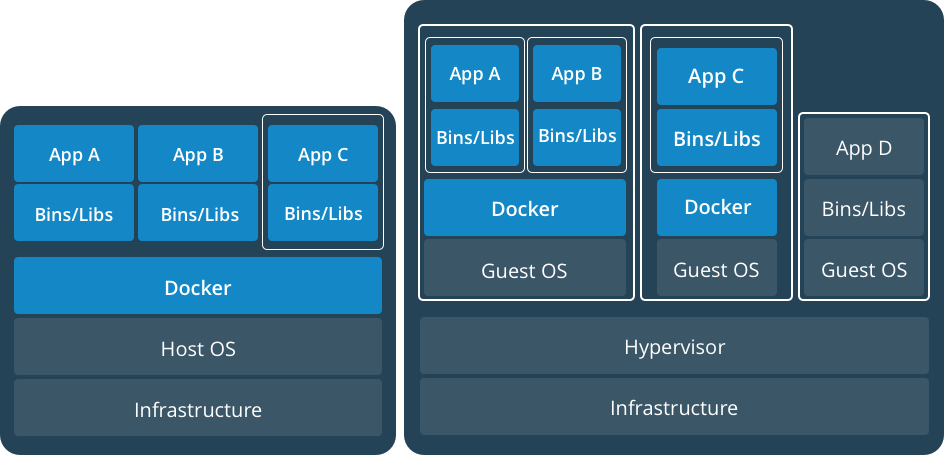
\includegraphics[width=7cm]{img/vm-container}
    \end{figure}    

    \end{multicols}
\end{frame}

\begin{frame}[fragile]{Installation}
    \begin{multicols}{2}
Sur une machine Ubuntu :
\begin{bashResized}{0.48}
sudo apt install docker
sudo systemctl start docker
\end{bashResized}
    \columnbreak
    
Sur MacOS ou Windows :
\begin{bashResized}{0.48}
Installer Docker Desktop :
https://www.docker.com/
\end{bashResized}
    \end{multicols}

    Pour pouvoir lancer des commandes docker sans privilèges :
\begin{bash}
sudo usermod -aG docker <username>
\end{bash}
\end{frame}

\begin{frame}[fragile]{Utilisation}
    Puis ensuite pour tester :
\begin{bash}
docker pull python
docker run -it python
\end{bash}

    \begin{figure}
        \centering
        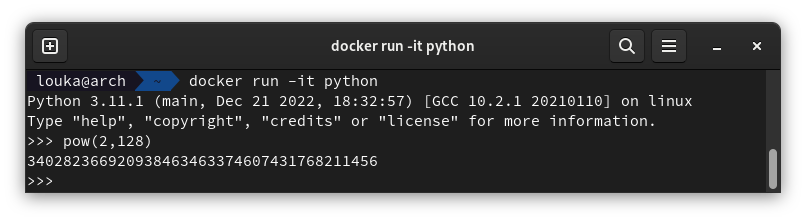
\includegraphics[width=\textwidth]{img/docker-test.png}
    \end{figure}
\end{frame}

\section{Docker Swarm}

% Multicol frame
\begin{frame}{Présentation}
    \begin{multicols}{2}
    Docker Swarm est un outil d'orchestration permettant de créer et gérer des clusters de
    machines physiques ou virtuelles hébergeant une application. C'est un outil intégré à Docker.

    L'interêt principal d'un cluster Swarm est la haute disponibilité que cela procure pour
    l'application.

    \columnbreak
    \begin{figure}
        \centering
        
\includegraphics[width=4cm]{img/swarm}
    \end{figure}

    \end{multicols}
\end{frame}

\begin{frame}{Terminologie}
    \begin{multicols}{2}
        \begin{itemize}
            \item Éléments d'un cluster \arrow \emph{Noeuds (nodes)}
            \item Cluster \arrow \emph{Manager(s) + Workers}
            \item Workers \arrow \emph{Exécution}
            \item Managers \arrow \emph{Orchestration}
        \end{itemize}
    \columnbreak
        \begin{figure}
            \centering
            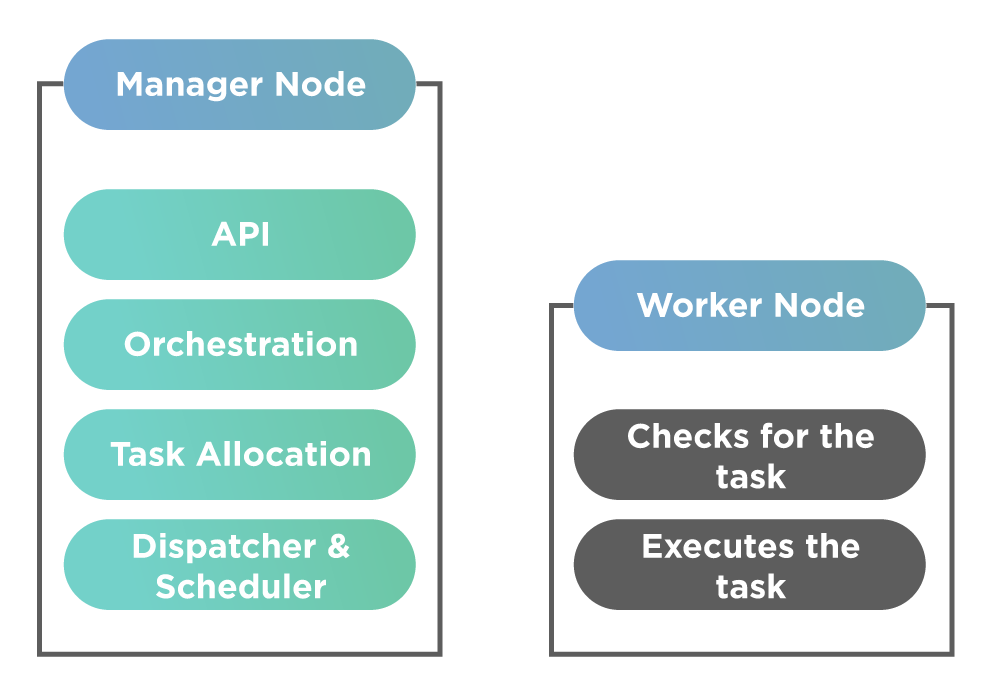
\includegraphics[width=0.5\textwidth]{img/manager}
        \end{figure}
    \end{multicols}
\end{frame}

\begin{frame}{Schéma d'un cluster}
    \begin{figure}
        \centering
        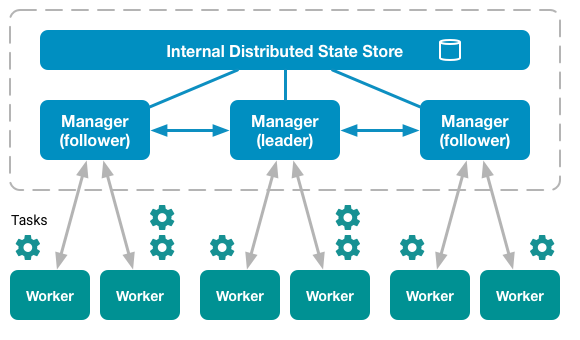
\includegraphics[width=0.85\textwidth]{img/swarm-network}
    \end{figure}
\end{frame}

\begin{frame}{Pourquoi utiliser Swarm ?}
    \begin{multicols}{2}
        \begin{itemize}
            \item Scalabilité
            \item Équilibrage de charges automatique
            \item Retour à l'état souhaité
            \item Mise en réseau multi-hôtes
            \item Sécurité
        \end{itemize}
    \columnbreak
        \begin{figure}
            \centering
            
\includegraphics[width=0.24\textwidth]{img/scalability}
            
\includegraphics[width=0.24\textwidth]{img/load-balancing}
        \end{figure}
    \end{multicols}
\end{frame}

\section{Démonstration}

% docker service create --name my_web --replicas 3 --mount type=bind,source=/,target=/usr/share/nginx/html --publish 8080:80 nginx
\begin{frame}[fragile]{Création du cluster}
Se connecter sur \verb:docker-manager: puis lancer:
\begin{bash}
docker swarm init
\end{bash}
\end{frame}

\begin{frame}[fragile]{Ajout des nodes}
Se connecter sur \verb:docker-worker1: et \verb:docker-worker2: puis lancer:
\begin{bash}
docker swarm join --token <token> <manager ip>:2377
\end{bash}
\end{frame}

\begin{frame}[fragile]{Création du service web}
Se connecter sur \verb:docker-manager: puis lancer:
\begin{bash}
docker service create --name my_web --replicas 3 \
    --mount type=bind,source=/,target=/usr/share/nginx/html \
    --publish 8080:80 nginx
\end{bash}
\end{frame}

\begin{frame}[fragile]{Tests}
Depuis l'hôte:
\begin{bash}
for i in `seq 1 10`; do curl http://<any ip>:8080/index.html; done
\end{bash}
\end{frame}


\section{Conclusion}

% Q&A
\begin{frame}[standout]
    \Huge\textsc{Merci de votre écoute}
    \vfill
    \LARGE\textsc{Questions ?}
\end{frame}

\section*{Bibliographie}

\begin{frame}[allowframebreaks]
    \frametitle{Références}
    \nocite{*}
    \bibliographystyle{acm}
    \bibliography{bibliography}
\end{frame}

\end{document}



%\bibliographystyle{unsrt}
%\bibliography{bibs/sample}
%\addcontentsline{toc}{chapter}{Bibliographie}

\end{document}
